\begin{wrapfigure}[0]{r}[0cm]{4cm}
	\vspace{-6cm}
  	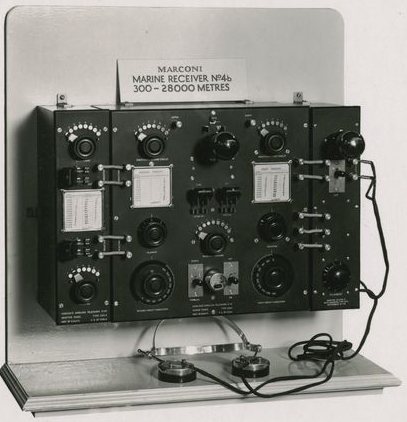
\includegraphics[scale=0.35]{Betriebsarten/Bilder/receiver.jpg}
 	\vspace{-6cm}
	\end{wrapfigure}

\section*{Theorie- und Prüfungsfragen}




\begin{enumerate} 
	\item[1] \emph{\textbf{TE309}} Um RTTY-Betrieb durchzuführen benötigt man außer einem Transceiver beispielsweise ...
	\begin{enumerate}
	\itemsep1pt\parskip0pt\parsep0pt
		\item[A] einen Fernschreiber.
		\item[B] einen RTTY-Controller.
		\item[C] eine Zusatzeinrichtung, die RTTY-Signale umwandelt und anschließend zwischenspeichert.
		\item[D]  einen PC mit Soundkarte und entsprechender Software.
		\loesung{Lösung D}
	\end{enumerate} 
	\item[2] \emph{\textbf{TE308}}  Eine Packet-Radio-Mailbox ist ...
	\begin{enumerate}
	\itemsep1pt\parskip0pt\parsep0pt
		\item[A] die Softwaresteuerung einer automatischen Funkstelle.
		\item[B] eine fernbedient oder automatisch arbeitende Funkstelle die Internetnachrichten zwischenspeichert.
		\item[C] eine Zusatzeinrichtung die E-Mails umwandelt und anschließend zwischenspeichert.
		\item[D] ein Rechnersystem bei dem Texte und Daten über Funk eingespeichert und abgerufen werden können.
		\loesung{Lösung D}
	\end{enumerate} 
	\item[3] \emph{\textbf{TE305}}  Was bedeutet im Prinzip „Packet Radio“?
	\begin{enumerate}
	\itemsep1pt\parskip0pt\parsep0pt
		\item[A] Die Daten werden paketweise (stoßweise) gesendet.
		\item[B] Die Daten werden in der Mailbox in Paketen aufbewahrt.
		\item[C] 8-Bit-weise parallel gepackt gesendet.
		\item[D] zu 8 Bit gepackt und dann gesendet.
		\loesung{Lösung A}
		\end{enumerate} 
	\item[4] \emph{\textbf{TE304}}  Was versteht man bei Packet Radio unter einem TNC (Terminal Network Controller)? Ein TNC ...
	\begin{enumerate}
	\itemsep1pt\parskip0pt\parsep0pt
		\item[A] ist ein Modem (Modulator und Demodulator) für digitale Signale.
		\item[B] wandelt nur die Töne in digitale Daten und schickt diese an den PC.
		\item[C] wandelt nur die Töne in digitale Daten und schickt diese an den Sender.
		\item[D] besteht aus einem Modem und dem Controller für die digitale Aufbereitung der Daten.
		\loesung{Lösung D}
		\end{enumerate} 	
	\item[5] \emph{\textbf{TE303}}  Welche NF-Zwischenträgerfrequenzen werden in der Regel in Packet Radio bei 1200 Baud benutzt?
	\begin{enumerate}
	\itemsep1pt\parskip0pt\parsep0pt
		\item[A] 1200 / 2200 Hz
		\item[B] 850 / 1200 kHz
		\item[C] 500 / 1750 Hz
		\item[D] 300 / 2700 Hz
		\loesung{Lösung A}
		\end{enumerate} 
	\item[6] \emph{\textbf{TE306}}  Was versteht man unter 1k2-Packet-Radio?
	\begin{enumerate}
	\itemsep1pt\parskip0pt\parsep0pt
		\item[A] Man arbeitet mit einem einzelnen Ton von 1200 Hz.
		\item[B] Die Frequenz am Packet Radio Eingang beträgt 1200 Hertz.
		\item[C] Die Übertragung erfolgt mit 1200 Baud.
		\item[D] Die Daten werden in Paketen von 1200 Bits übertragen.
		\loesung{Lösung C}
		\end{enumerate} 
	\item[7] \emph{\textbf{TE302 }}  Welche HF-Bandbreite beansprucht ein 9600-Baud-FM-Packet-Radio-Signal?
	\begin{enumerate}
	\itemsep1pt\parskip0pt\parsep0pt
		\item[A] 12,5 kHz 
		\item[B] 20 kHz 
		\item[C] ca. 6,6 kHz
		\item[D] ca. 3 kHz
		\loesung{Lösung B}
		\end{enumerate} 
	\item[8] \emph{\textbf{TE312}} Wie heißt die Übertragungsart mit einem Übertragungskanal, bei der durch Umschaltung abwechselnd in beide Richtungen gesendet werden kann?
	\begin{enumerate}
	\itemsep1pt\parskip0pt\parsep0pt
		\item[A] Simplex
		\item[B] Duplex 
		\item[C] Halbduplex
		\item[D] Vollduplex
		\loesung{Lösung C}
		\end{enumerate} 
	\item[9] \emph{\textbf{TE308}} Was versteht man unter APRS im Amateurfunk?
	\begin{enumerate}
	\itemsep1pt\parskip0pt\parsep0pt
		\item[A] Es ist ein automatisches Positionsmeldesystem.
		\item[B] Es bedeutet eine automatische Adressierung bei Packet Radio.
		\item[C] Es dient zur automatischen Verbindung mit dem Zielrufzeichen.
		\item[D] Es dient zur automatischen Streckenführung einer mobilen PR-Station.
		\loesung{Lösung A}
		\end{enumerate} 
	\item[10] \emph{\textbf{TE311}}Welches der folgenden digitalen Übertragungsverfahren hat die geringste Bandbreite?
	\begin{enumerate}
	\itemsep1pt\parskip0pt\parsep0pt
		\item[A] RTTY
		\item[B] Pactor
		\item[C] PSK31
		\item[D] Packet Radio
		\loesung{Lösung C}
		\end{enumerate} 
	\item[11] \emph{\textbf{TE301}}Welche Sendearten sind für QRP-DX-Betrieb auf Kurzwelle am besten geeignet?
	\begin{enumerate}
	\itemsep1pt\parskip0pt\parsep0pt
		\item[A] CW, Pactor, PSK31
		\item[B] RTTY, SSB, FM
		\item[C] Pactor, RTTY, SSB
		\item[D] SSTV, PSK31, AM
		\loesung{Lösung A}
		\end{enumerate} 
	\item[12] \emph{\textbf{TE312}}Wie wird ein SSTV-Signal beurteilt? Es wird beurteilt mit ...
	\begin{enumerate}
	\itemsep1pt\parskip0pt\parsep0pt
		\item[A] R, S und „V" für Video-Qualität, V in 5 Stufen
		\item[B] V, S, T, mit „V" für Video-Qualität, V in 5 Stufen
		\item[C] mit „S“ für Signalstärke und „V" für Video-Qualität, S und V in 9 Stufen
		\item[D] R, S, T und einer zusätzlichen Bildbewertung
		\loesung{Lösung A}
		\end{enumerate} 
\end{enumerate}



